\chapter{Perspectives}
\label{chap:perspectives}
In this Chapter future research topics in the domain of tracking at high luminosity colliders will be 
presented.
 The search for thin and edgeless pixel sensors will continue with new productions which will 
 be tested throughly after irradiation to fluences expected at the HL-LHC (Section~\ref{sec:PerspPixels}). 
 The data extracted from beam test measurements of irradiated 
 pixel modules can be used to improve the modelling of radiation damage (Section~\ref{sec:PerspTCAD}).
 Some comments will be made on the importance of optimising the 
algorithm of clustering, vertexing, tracking and flavour tagging when the pixel sensors 
will be severely hit by radiation damage (Section~\ref{sec:algos}).
A novel solutions for thermal management and mechanical structures for  future silicon detector system 
will be presented in Section~\ref{sec:microchannels}.



\section{Radiation Hard Pixels Sensors}
\label{sec:PerspPixels}
The results for  thin pixel detectors presented in~\ref{sec:PAE2pixels} and for edgeless 
ones in~\ref{sec:edgeless} are very promising in terms of hit-efficiency after irradiation of the former 
and of performance at the detector edge for the latter. The next step is to prove that 
thin edgeless pixel detectors are suited for the HL-LHC phase of ATLAS. For this a new 
planar pixel production was realised~\cite{SabinaTrentoWS2017} on high resistivity 6" $p-$bulk material 
wafers; sensor wafers active thickness is as thin as 100~$\mu$m. Edgeless pixels detectors 
compatible with the FE-I4 chip  have been designed, featuring a pixel-to-edge distance 
as low as 50~$\mu$m. As we write some of these new pixel sensors prototypes are being bump-bonded 
to FE-I4 chip and should be tested before the end of the year.
Sensors compatible with the new RD53A chip prototype were included in the production, 
with both 50~$\mu$m~$\times$~50~$\mu$m  and 25~$\mu$m~$\times$~100~$\mu$m pitch pixels. 
The plan is to have some of them connected to  the  RD53A chip and test them on beam 
next year.

For both FE-I4 and RD53A modules the plan is to irradiate them at fluences of the order of
 1.0$\times10^{16}$~n$_{\rm eq}$/cm$^2$ and retest them on beam after irradiation. 
This time, thanks to the deposition of   a layer of Benzocyclobutene (BCB) on the readout chip surface at 
wafer level it will be possible to verify the efficiency at the detector edge after those very large fluences. 

Diodes, test-structures and baby detectors will be irradiated too, to be then studied in laboratory 
to extract valuable information to be used to better understand and model the effects of the radiation 
damage in silicon.

\section{Improved TCAD and Monte Carlo Pixels Simulations}
\label{sec:PerspTCAD}

Concerning radiation damage modelling for TCAD based simulations, as already mentioned in 
Chapter~\ref{chap:TCAD} all of the radiation damage models work fine for certain type of sensors and 
conditions, even more  if they were tuned for specific measurements. 
A nice review of the situation can be found in~\cite{GregorVertex2016}. 
Despite the fact that the detector properties after irradiation depend on the initial detector material, particle  
and energy of the irradiation step (one recent example is here~\cite{Allport2016}), an effort to 
define a minimal set of radiation damage models should be pursued. This is very important in 
view of the HL-LHC phase of ATLAS, where a mix of several hadrons with different 
energies spectra will be responsible for the radiation damage to the tracking detector.
Data from beam test campaigns will be fundamental, but also collision data from LHC Run~2~and~3 
will be valuable for this purpose; indeed, given the excellent luminosity performance of LHC as we write, 
effects due to radiation damage are already visible in the actual ATLAS tracker, as 
shown in Chapter~\ref{chap:digi}.


During the Phase-II  data taking of ATLAS it will be important to update often  the  Monte Carlo 
simulations, following the changing conditions of the pixel detector due to the accumulated fluence. 
Using more accurate radiation damage models in combination with a good knowledge of  the composition in 
energy and particles of the radiation received by the detector, through an approach as the one outlined 
in Chapter~\ref{chap:digi}, reliable simulation of the  the detector behaviour will be prepared.   

Accurate and detailed simulations of the pixel detectors after large irradiation fluences will be 
also important during the preparation of the data taking at the HL-LHC but also during the actual 
and next LHC Run. Clustering, tracking, vertexing and flavour tagging algorithms will need to be updated 
to assure they will still deliver high performance on physics objects, even with a damaged tracking 
detector. 

\section{ITk Performance Optimisation}
\label{sec:algos}

The possibilities offered by the dataset foreseen at the HL-LHC are many. 
For the search of Higgs boson decaying to second generation fermions, for other Higgs sector 
studies, and for many New Physics (NP) scenarios not only outstanding tracking and vertexing of charged 
particles are needed but  excellent reconstruction of jets is mandatory  too. 
To achieve the highest possible performance tracker information should be exploited at maximum 
together with calorimeter. 
The chief advantages of integrating tracking and calorimetric information into one hadronic reconstruction
step are~\cite{ATLASParticleFlow}:
\begin{itemize}
\item the momentum resolution of the tracker is significantly better than the energy resolution of the
calorimeter for low-energy charged particles;
\item the angular resolution of a single charged particle, reconstructed using the tracker is much better
than that of the calorimeter;
\item a better association of low $p_T$ charged particles to the right jet, and
\item a better association to the correct production vertex so important reduction of degradation due to pile-up  
\end{itemize}
It is clear that the ATLAS Inner Tracker is of the uttermost importance for all
the searches and studies of ATLAS. 
As it was already mentioned in the previous Section, clustering, tracking, vertexing and flavour tagging 
algorithms will need to be updated to reflect the changes in the inner tracker detector.

A good  test case to 
study the radiation damage impact  on physics  performance and analysis is offered by 
the $H\to\b\bbar$ decay channel; 
this is a study case that is in 
perspective very important given the excellent luminosity performance of LHC as we write.

\subsection{Impact of Radiation Damage on Higgs Analysis}
\label{sec:raddamHiggs}
The decay of the SM Higgs boson to pairs of  $b-$quarks is expected to have a branching ratio of 58\% 
for a mass of the Higgs boson $m_H$ of 125~GeV~\cite{ATLASHbb2017}.
At the LHC the very large backgrounds arising from multi-jet production make the inclusive search
extremely challenging. Careful reconstruction of secondary vertices is needed, to ensure 
the correct association of $b-$vertices to the same primary vertex, rejecting the huge QCD $\b\bbar$ 
background, but also to identify the flavour of the jets with good efficiency and high purity. 
All these ingredients of course strongly depend on the tracker performance. 
As shown in Chapter~\ref{chap:digi} radiation damage effects can already be measured in the actual 
detector. Hence it would be very interesting to produce Monte Carlo simulations with a pixel 
detector at a reduced charge collection efficiency and then process them using un-optimised 
tracks reconstruction algorithms to see which is the impact of silicon pixel sensors hit by radiation 
damage on jets flavour tagging and then on the $H\to\b\bbar$ analysis itself. 
Two scenarios are possible:
\begin{enumerate}
 \item if algorithms performance are still acceptable then scenarios with different levels of charge collection 
 losses can be simulated and analysed, to understand when the  algorithms will need to be optimised;
 \item if there is the need to retune algorithms a study of their performance should be performed
  as a function of the integrated fluence by the pixel detector; this could help in assessing better 
  the systematic uncertainties to jet reconstruction and flavour tagging.
\end{enumerate}



\section{Microchannel Cooling for the ITK Pixels}
\label{sec:microchannels}

The need of highly performing cooling systems using small amounts of fluids is nowadays mandatory for silicon detectors in fundamental physics and in general for all the applications requiring a high level of miniaturisation. There are indeed two conflicting trends concerning many modern devices: the need to dissipate increasing amounts of heat and and the quest for more compact and lightweight designs.

One very promising solution consists in exploiting CO$_2$ latent and sensible heat, rather than sensible 
heat only. 
Indeed the cooling system for the ITk Strip and Pixel Detectors will be based on evaporating CO$_2$ in a 
liquid 
pumped cycle cooled by an external primary chilling source.  CO$_2$ cooling is chosen as this gives 
significant mass savings inside the detector due to the possibility of having smaller diameter tubing than 
conventional refrigerants or liquid cooling applications.


The two innermost barrel layers and the innermost endcap ring layer are placed inside an Inner Support 
Tube, allowing for their potential replacement. In contrast, the three outer barrel layers and three outer end-
cap ring layers are between the Inner Support Tube (IST) and the Pixel Support Tube (PST), and are, like 
the Strip Detector, designed to operate for the entire lifetime of the HL-LHC.

The replacement of the innermost layers of the ITk pixel detector could offer the possibility to move from 
a cooling system based on metal pipes to one based on microchannels etched in the silicon.

Channels with a hydraulic diameter below 1 mm are defined as microchannels. Microchannels have been etched on many materials, like Polyimide, Silica Glass, Quartz, Steel, Silicon, Copper, 
and more~\cite{KOSAR2010635}.
In Figure~\ref{fig:uChannels} a sketch of pixel detector module with micro channel cooling system integrated.
\begin{figure}[!htpb]
\centering
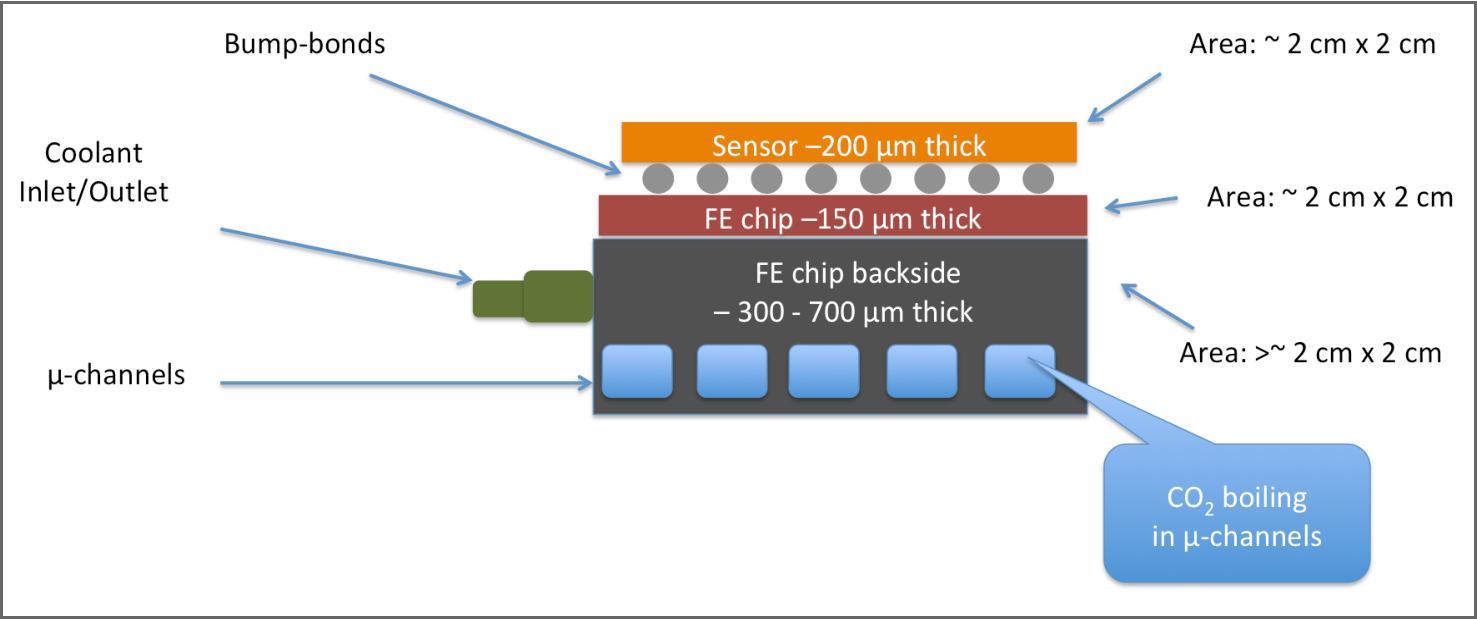
\includegraphics[width=1.0\textwidth]{uChannels.pdf}
\caption{\label{fig:uChannels}Schematic sketch of a pixel detector module with micro channel cooling system integrated.}
\end{figure}

The microchannels are etched on the backside of the unprocessed wafer that will be used for realising 
later the front-end chips. After the microchannels are etched a silicon oxide layer to seal them is grown. 
The opposite side of the wafer can be thinned down to the desired thickness before realising the 
readout circuitry. 

A cooling system based on CO$_2$ evaporating in microchannels etched in silicon   offers:
\begin{itemize}
\item very uniform and efficient heat removal; the channels position can be optimised to maximise the 
cooling efficiency;
\item reduction of all possible thermic transmission inefficiencies and  reflections to interfaces between 
materials with different thermal properties thanks to the fact that the cooling unit is made of silicon as the 
detector module;
\item for the same reason above mechanical stress due to thermal expansion will be minimised too, being 
the system more homogenous;
\item the system will be more lightweight in terms of material budget since made of silicon only, and 
the material distribution will be more uniform with respect to a stave with a metal pipe.
\end{itemize}


For the future LHCb vertex detector a microchannel based cooling system was 
proposed~\cite{1748-0221-8-04-P04004}. This is very promising since the LHCb experiment has 
a fixed target geometry and mass can be placed immediately outside active elements. 
For more classical collider experiments geometries like ATLAS the problem of having long barrel staves 
(500-1000~mm) dictates the need of connecting many cooling units together. Low mass and high 
pressure resistant connector are at the moment object of intense research. 

Within the {\it REFLECS} and {\it REFLECS2} projects~\cite{REFLECS} microchannels-based cooling units, 
created by etching silicon wafers, were created, with two scientific goals: realize cooling prototype units 
for the future ATLAS Inner Tracker (ITk); study the basics of the two-phase microfluidics. If the first research 
axe should be by now clear, for the second it must be said that at the moment a valid numerical model for 
the two-phase fluid flowing in microchannels is missing~\cite{KIM201474}, especially in high pressure applications (50-200 
bars and more).
Once etched the silicon wafers were sealed by a pyrex wafer through anodic bonding. 
Figure~\ref{fig:reflecs} shows details of the wafers produced at FBK within the project. 
\begin{figure}[!htpb]
\centering
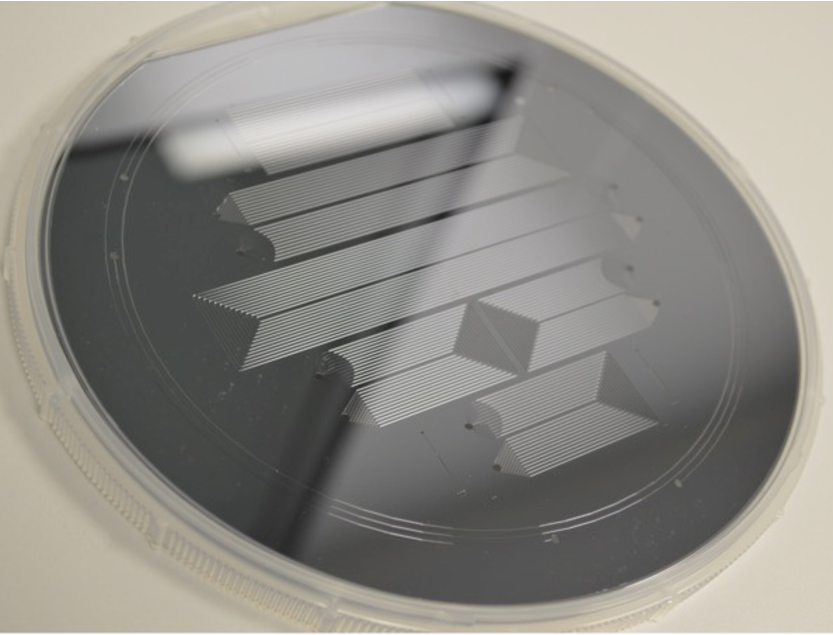
\includegraphics[width=0.49\textwidth]{Wafer.pdf}
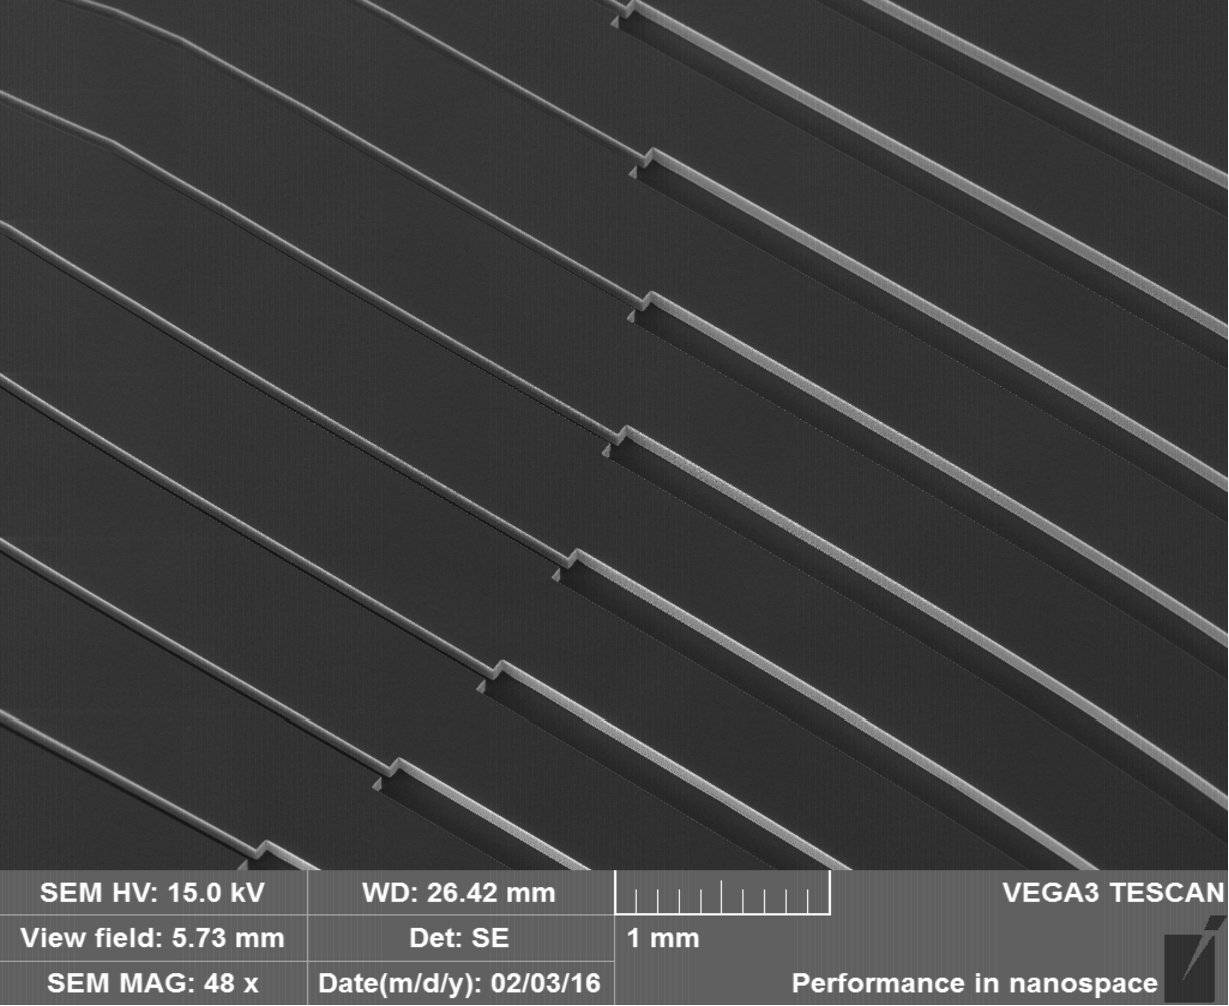
\includegraphics[width=0.46\textwidth]{restrictions.pdf}
\caption{\label{fig:reflecs}Silicon etched microchannels. (left) Wafer of microchannels prototypes, 
sealed by a pyrex wafer. (right) Channel restrictions to favour the start of the fluid boiling; channels are 
120~$\mu$m deep and 60~(200)~$\mu$m in the narrow (wide) section.}
\end{figure}
Another research axis within these projects is the idea of using 3D printed ceramics connectors, 
exploiting the good thermal specifications of ceramics. 

The first samples from the REFLECS2 project wafers were cut and they will be soon connected 
to a CO$_2$ plant for tests, using a high resolution camera to study the bubbles formation and the 
biphasic flow. These data will be valuable to better understand the flow and boiling of two-phase fluid 
in microchannels at high pressure. 

These studies could lead to a microchannel based cooling stave for the replacement of the innermost 
ITk layers.

\chapter*{Summary}
\addcontentsline{toc}{chapter}{Summary}
In this report, prepared  to obtain the  ``Habilitation \`a Diriger des Recherches'', I have 
presented the highlights of my work  after getting my PhD degree. 
All my research activities had in common the development of silicon tracking systems for high luminosity 
colliders, first for \epem machines then for hadron colliders. 

I have started focusing on strip detectors (Chapter~\ref{chap:SLIM5}) for Linear Collider and Super 
Flavour Factories experiments,  working on the sensor characterisation and the beam test data simulation, 
reconstruction and analysis. 

Later, after moving to the  ``Laboratoire de Physique Nucl\'eaire et de Hautes Energies'' (LPNHE), to 
work with the local ATLAS group, my focus shifted on pixel detectors for the High Luminosity LHC 
experiments. Here I have contributed at the research and development of thin and edgeless 
pixel sensors, participating in all the R\&D steps, from sensor design conception and simulations to 
the tests on beam of prototypes (Chapters~\ref{chap:TCAD} and~\ref{chap:ITk}). 

The knowledge I gained about radiation damage and TCAD simulations allowed me to make important 
contributions to the understanding and the simulation of the actual ATLAS pixel detector system 
(Chapter~\ref{chap:digi}). 

I am very eager to continue my research on high luminosity silicon trackers development, 
a field that I wanted and had the opportunity to join 10 years ago. 
With the ITk pixel detector construction about to start in two years it is time to focus on pixel 
module construction, to which I will contribute thanks to my experience. But other than 
pixel sensor modules I want also to pursue innovative solutions for pixel detector services, 
like the micro-channels based cooling solution.

Beyond pixel detector construction itself, I see myself participating to the preparation of the 
data taking at the HL-LHC, working on the understanding of the expected performance of the 
new ATLAS tracker in terms of tracking, vertexing and flavour tagging. The combination of my 
expertise in pixel detector characterisation, simulation and data analysis, should allow me 
to make important contributions to these crucial tools for precision measurements and discoveries. 

Within the LPNHE ATLAS group I think I can fulfil my research program, including possibly 
a contribution to future studies on Higgs boson decays, in preparation for the analysis 
at the High Luminosity LHC.

